\documentclass[tikz,convert={outfile=fonctions.png}]{standalone}

    \usepackage[utf8]{inputenc}

\begin{document}
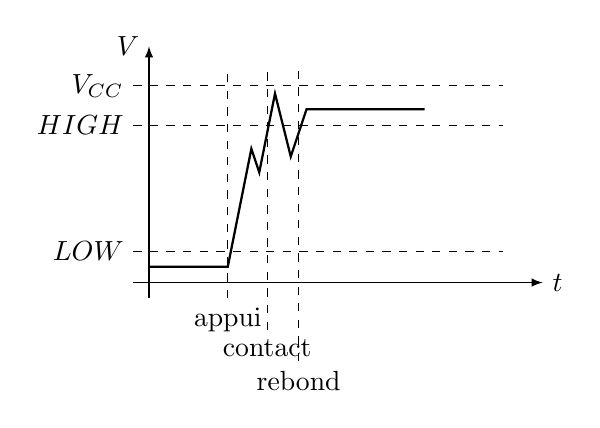
\begin{tikzpicture}[>=latex]

    \draw[->] (-.2,0) -- (5,0) node[right] {$t$};
    \draw[->] (0,-.2) -- (0,3) node[left] {$V$};

    \draw[dashed] (-.2,.4) node[left] {$LOW$} -- (4.5,.4);
    \draw[dashed] (-.2,2) node[left] {$HIGH$} -- (4.5,2);
    \draw[dashed] (-.2,2.5) node[left] {$V_{CC}$} -- (4.5,2.5);

    % signal
    \draw[thick] (0,.2) -- (1,.2) -- (1.3,1.7) -- (1.4,1.4) -- (1.6,2.4) -- (1.8,1.6) -- (2,2.2) -- (3.5,2.2);

    % appui
    \draw[dashed] (1,-.2) node[below] {appui} -- (1,2.7);
    \draw[dashed] (1.5,-.6) node[below] {contact} -- (1.5,2.7);
    \draw[dashed] (1.9,-1) node[below] {rebond} -- (1.9,2.7);
   
\end{tikzpicture}
\end{document}

